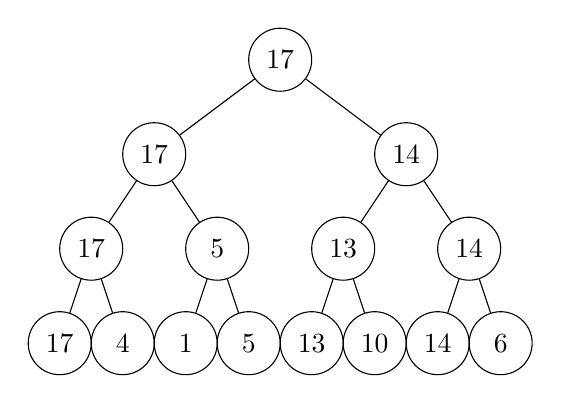
\begin{tikzpicture}[scale=0.8]
\tikzstyle{every node}=[draw,shape=circle,minimum size=0.8cm];
\node {17}[sibling distance=4cm]
child { node {17}[sibling distance=2cm]
	child {
		node {17}[sibling distance=1cm]
		child { node {17} }
		child { node {4} }
	}
	child {
		node {5}[sibling distance=1cm]
		child { node {1} }
		child { node {5} }
	}
}
child { node {14}[sibling distance=2cm]
	child {
		node {13}[sibling distance=1cm]
		child { node {13} }
		child { node {10} }
	}
	child {
		node {14}[sibling distance=1cm]
		child { node {14} }
		child { node {6} }
	}
};
\end{tikzpicture}